\documentclass[a4paper, 11pt]{article}
\usepackage{comment} % enables the use of multi-line comments (\ifx \fi) 
\usepackage{fullpage} % changes the margin
\usepackage{graphicx}
\usepackage{fancyvrb,xcolor}
\usepackage{listings}
\usepackage{color}
\usepackage[hyphenbreaks]{breakurl}
\usepackage[hyphens]{url}
\usepackage[margin=3cm]{geometry}

\definecolor{dkgreen}{rgb}{0,0.6,0}
\definecolor{gray}{rgb}{0.5,0.5,0.5}
\definecolor{mauve}{rgb}{0.58,0,0.82}
\usepackage{float}

\usepackage{caption}
\DeclareCaptionFont{white}{\color{white}}
\DeclareCaptionFormat{listing}{\colorbox{gray}{\parbox{\textwidth}{#1#2#3}}}
\captionsetup[lstlisting]{format=listing,labelfont=white,textfont=white}

\lstset{
  language=Java,
  aboveskip=3mm,
  belowskip=3mm,
  showstringspaces=false,
  columns=flexible,
  basicstyle={\small\ttfamily},
  numbers=none,
  numberstyle=\tiny\color{gray},
  keywordstyle=\color{blue},
  commentstyle=\color{dkgreen},
  stringstyle=\color{mauve},
  breaklines=true,
  breakatwhitespace=true,
  tabsize=3
}
\graphicspath{ {images/} }

\begin{document}
%Header-Make sure you update this information!!!!
\noindent
\large\textbf{Assignment 2} \hfill \textbf{Hussam Hallak} \\
\normalsize CS532, Web Science, Spring 2017\hfill CS Master's Student \\
Old Dominion University, Computer Science Dept \hfill Prof: Dr. Nelson 

\section*{Question 1:}
1.  Write a Python program that extracts 1000 unique links from
Twitter.  You might want to take a look at:

http://adilmoujahid.com/posts/2014/07/twitter-analytics/

see also:

http://docs.tweepy.org/en/v3.5.0/index.html

https://github.com/bear/python-twitter

https://dev.twitter.com/rest/public

But there are many other similar resources available on the web.

\textbf{Note:}
Only Twitter API 1.1 is currently available; version 1
code will no longer work.

\textbf{Note:}
You need to verify that the final target URI (i.e.,
the one that responds with a 200) is unique.  You could have many
different shortened URIs for www.cnn.com (t.co, bit.ly, goo.gl,
etc.).  For example:


\begin{lstlisting}[language=bash,label=Command:, breakatwhitespace=〈false), caption=Command:]
$ curl -IL --silent https://t.co/DpO767Md1v | egrep -i "(HTTP/1.1|^location:)"
HTTP/1.1 301 Moved Permanently
location: https://goo.gl/40yQo2
HTTP/1.1 301 Moved Permanently
\end{lstlisting}
\burl{Location: https://soundcloud.com/roanoketimes/ep-95-talking-hokies-recruiting-one-week-before-signing-day}
\nolinebreak
\begin{lstlisting}[language=bash]
HTTP/1.1 200 OK
\end{lstlisting}



You might want to use the search feature to find URIs, or you can
pull them from the feed of someone famous (e.g., Tim O'Reilly).  If
you find something inappropriate for any reason you see fit, just
discard it and get some more links.  We just want 1000 links that
were shared via Twitter.

Hold on to this collection and upload it to github -- we'll use it
later throughout the semester.

\subsection*{Answer:}
The approach is divided into two steps:

1. Collect tweets with external links, parse them and save the unique external links in the file ``links.txt''. I wrote a python script to do that ``getlinks.py''. This python script must be run several times until 1000 links or more are collected (more duplicates are removed later in the second step).
The script asks the user to enter twitter username(s) to pull their last tweets that contain links. Twitter username(s) are passed to the program as command line argument(s). The program loops over all usernames and pulls their tweets that contain links. It follows all redirects until 200 OK is returned. It removes links that lead to other tweets, not external to Twitter. The program removes duplicates in the captured links and writes them to the file ``links.txt''.
Twitter API credentials are saved in a separate file, ``config.py''.
\lstinputlisting[language=Python, label=config.py, caption=The content of config.py]{Q1/config.py}

\lstinputlisting[language=Python, breakatwhitespace=〈false), label=getlinks.py, caption=The content of getlinks.py]{Q1/getlinks.py}

Running the Program: 
\lstinputlisting[language=bash, label=running getlinks.py, caption= Running getlinks.py to collects external links from cnn's tweets]{Q1/getlinks.run.txt}
The program created the file ``links.txt'' and stored the links in it. 

\textbf{Note:} The program discarded two of the captured links because they are not external. It shows what the discarded links are. 

After running the program enough times to extract tweets with links from different users, I collected 1405 links.

\lstinputlisting[language=bash, label=links.run.txt, caption= The number of external links extracted from tweets after multiple runs]{Q1/links.run.txt}

2. Ensuring that the extracted 1405 links are unique:
After running the program multiple times to extract enough links to have 1000 unique links, now we need to make sure that the extracted links from multiple runs are unique.

The script ``makeunique.py'' is a simple script that takes 2 command line arguments, an input file that we want to remove duplicated links from, and an output file to store unique links in.

\lstinputlisting[language=Python, label=makeunique.py, caption=The content of makeunique.py]{Q1/makeunique.py}

After running ``makeunique.py'' on ``links.txt'' and saving the output in ``uniquelinks.txt'', I got 1107 unique links out of the 1405 links in ``links.txt''. 298 links were duplicates.

\lstinputlisting[language=bash, label=running makeunique.py, caption= The number of unique links in links.txt saved in uniquelinks.txt]{Q1/uniquelinks.run.txt}

\subsection*{Included Files:}
config.py getlinks.py, makeunique.py, links.txt, uniquelinks.txt, getlinks.run.txt

\section*{Question 2:}
2.  Download the TimeMaps for each of the target URIs.  We'll use the ODU 
Memento Aggregator, so for example:

\begin{lstlisting}[language=bash,label=Command:, breakatwhitespace=〈false), caption=Command:]
URI-R = http://www.cs.odu.edu/

URI-T = http://memgator.cs.odu.edu/timemap/link/http://www.cs.odu.edu/

or:

URI-T = http://memgator.cs.odu.edu/timemap/json/http://www.cs.odu.edu/
\end{lstlisting}
(depending on which format you'd prefer to parse)

Create a histogram* of URIs vs. number of Mementos (as computed
from the TimeMaps).  For example, 100 URIs with 0 Mementos, 300
URIs with 1 Memento, 400 URIs with 2 Mementos, etc.  The x-axis
will have the number of mementos, and the y-axis will have the
frequency of occurence.

* = https://en.wikipedia.org/wiki/Histogram

What's a TimeMap?  

See: http://www.mementoweb.org/guide/quick-intro/

And the week 4 lecture. 

\subsection*{Answer:}
The approach is divided into three steps:

1. Downloading the TimeMaps for each of the target URIs using the ODU 
Memento Aggregator. I wrote a python script to do that ``downloadtimemapsjson.py''. The script takes three command line arguments, an input file that has the links for which we want to download the TimeMaps ``uniquelinks.txt'', an output file to store the downloaded TimeMaps, ``timemap.jsonx'' where ``x'' is a number that identifies the timemap (e.g., 1, 2, 3, ...), and another output file, ``uniquelinkswithmemes.txt'', to store the unique links with mementos in.

\textbf{Note:} The number of output files named , ``timemap.jsonx'' may not be the same as the number of links in the input file ``uniquelinks.txt''. The reason is because not all links have mementos.

\textbf{Note:} An interesting discovery is that, sometimes, links with certain query string variables, GET variables, will make our results inaccurate because they have no mementos for the link as it is, however, if these variables are removed, the page has mementos. Some websites add these arguments so they can log where the user came from to visit their page.

Example:
this link is coming back with 404 error code, no mementos!

\burl{http://memgator.cs.odu.edu/timemap/link/http://www.bbc.co.uk/news/business-37047416?utm_source=twitterfeed&utm_medium=twitter}

The original link comes with 200 OK:

\burl{http://www.bbc.com/news/business-37047416?utm_source=twitterfeed&utm_medium=twitter}


\lstinputlisting[language=bash, label=bbnocmemes, caption=This shows that the page has no mementos, breakatwhitespace=〈false)]{Q2/bbcnomemes.txt}
\noindent
\textbf{Let's remove the string that contains these arguments:}
\begin{lstlisting}
?utm_source=twitterfeed&utm_medium=twitter
\end{lstlisting}
\textbf{Now it's time to see if there are any mementos for this link:}

\noindent
\burl{http://www.bbc.co.uk/news/business-37047416}
\lstinputlisting[language=bash, label=bbcmemes, caption=The mementos for our BBC link without the arguments, breakatwhitespace=〈false)]{Q2/bbcmemes.txt}


Note: It is clear that the page without the arguments has many mementos, however there is no telling which arguments to remove in each and every extracted link to prevent this case, but since we discovered this one, I am going to quickly remove it from all extracted links in ``uniquelinks.txt'' using this find and replace command:
\begin{lstlisting}[language=bash, breakatwhitespace=〈false), label=Command, caption=Command: Removing GET arguments]
sed -i 's/utm_source=twitterfeed&utm_medium=twitter//g' uniquelinks.txt

root@ima-app:/var/www/Hussam# sed -i 's/utm_source=twitterfeed&utm_medium=twitter//g' uniquelinks.txt
root@ima-app:/var/www/Hussam# cat uniquelinks.txt | grep "utm_source=twitterfeed&utm_medium=twitter"
root@ima-app:/var/www/Hussam#
\end{lstlisting}

\textbf{Syntax:}

sed -i 's/old/new/g' file.txt

\textbf{The command:}

sed: Stream Editor

\textbf{Options:}

-i: in-place (Save the result in the same file)

\textbf{Arguments:}

s: substitute

old: old string

new: new string

g: global (Replace all occurrences)

file.txt: file name

\lstinputlisting[language=python, label=downloadtimemapsjson.py, caption=The content of downloadtimemapsjson.py, breakatwhitespace=〈false)]{Q2/downloadtimemapsjson.py}

\begin{lstlisting}[language=bash, breakatwhitespace=〈false), label=Command, caption=Running downloadtimemapsjson.py]
root@ima-app:/var/www/Hussam# python downloadtimemapsjson.py uniquelinks.txt timemap.json uniquelinkswithmemes.txt
\end{lstlisting}

Now I have 445 links with mementos out of the original 1107 unique links in the input file.

\begin{lstlisting}[language=bash, breakatwhitespace=〈false), label=Command, caption=Links with mementos:]
root@ima-app:/var/www/Hussam# cat uniquelinks.txt | wc -l
1107
root@ima-app:/var/www/Hussam# cat uniquelinkswithmemes.txt | wc -l
445
root@ima-app:/var/www/Hussam# ls timemap.json* | wc -l
445
\end{lstlisting}

2. Parse the downloaded TimeMaps, JSON files, to find the number of mementos for each URI that has a TimeMap. I wrote a Python script, ``parsejsontimemap.py'', to do that. The script loops over all TimeMaps' files ``timemap.jsonx'' and parses them to find the number of mementos for each link. The program saves the results in a file as output, ``timemapreport.txt''. This is the file that we will use to generate our histogram in R in the next step.

\lstinputlisting[language=python, label=parsejsontimemap.py, caption=The content of parsejsontimemap.py, breakatwhitespace=〈false)]{Q2/parsejsontimemap.py}

\begin{lstlisting}[language=bash, breakatwhitespace=〈false), label=Command, caption=Running parsejsontimemap.py]
root@ima-app:/var/www/Hussam# python parsejsontimemap.py timemap.json timemapreport.txt
root@ima-app:/var/www/Hussam# cat timemapreport.txt | wc -l
445
\end{lstlisting}

3. Now we are ready to generate the histogram for URIs vs. the number of Mementos in R.

This line of code reads the data in the file and stores it in the vector timemaps\_data.
\begin{lstlisting}
> timemaps_data <- read.table("C:/R/timemapreport.txt", header=F, sep="\t")
\end{lstlisting}

This line of code defines a variable max\_num and assigns the maximum value in the vector timemaps\_data to it.
\begin{lstlisting}
> max_num <- max(timemaps_data)
\end{lstlisting}

This line of code creates a histogram for timemaps\_data  with fire colors, sets bin = 1 so each number is in its own group, makes x axis range from 0 to max\_num, disables right-closing of cell intervals, sets heading, changes the label of the x-axis, and makes y-axis labels horizontal
\begin{lstlisting}
> hist(timemaps_data[,1], col=heat.colors(max_num), breaks=max_num, xlab="Number of Mementos", xlim=c(0,max_num), right=F, main="Mementos Histogram", las=1)
\end{lstlisting}

\begin{figure}[H]
\centering
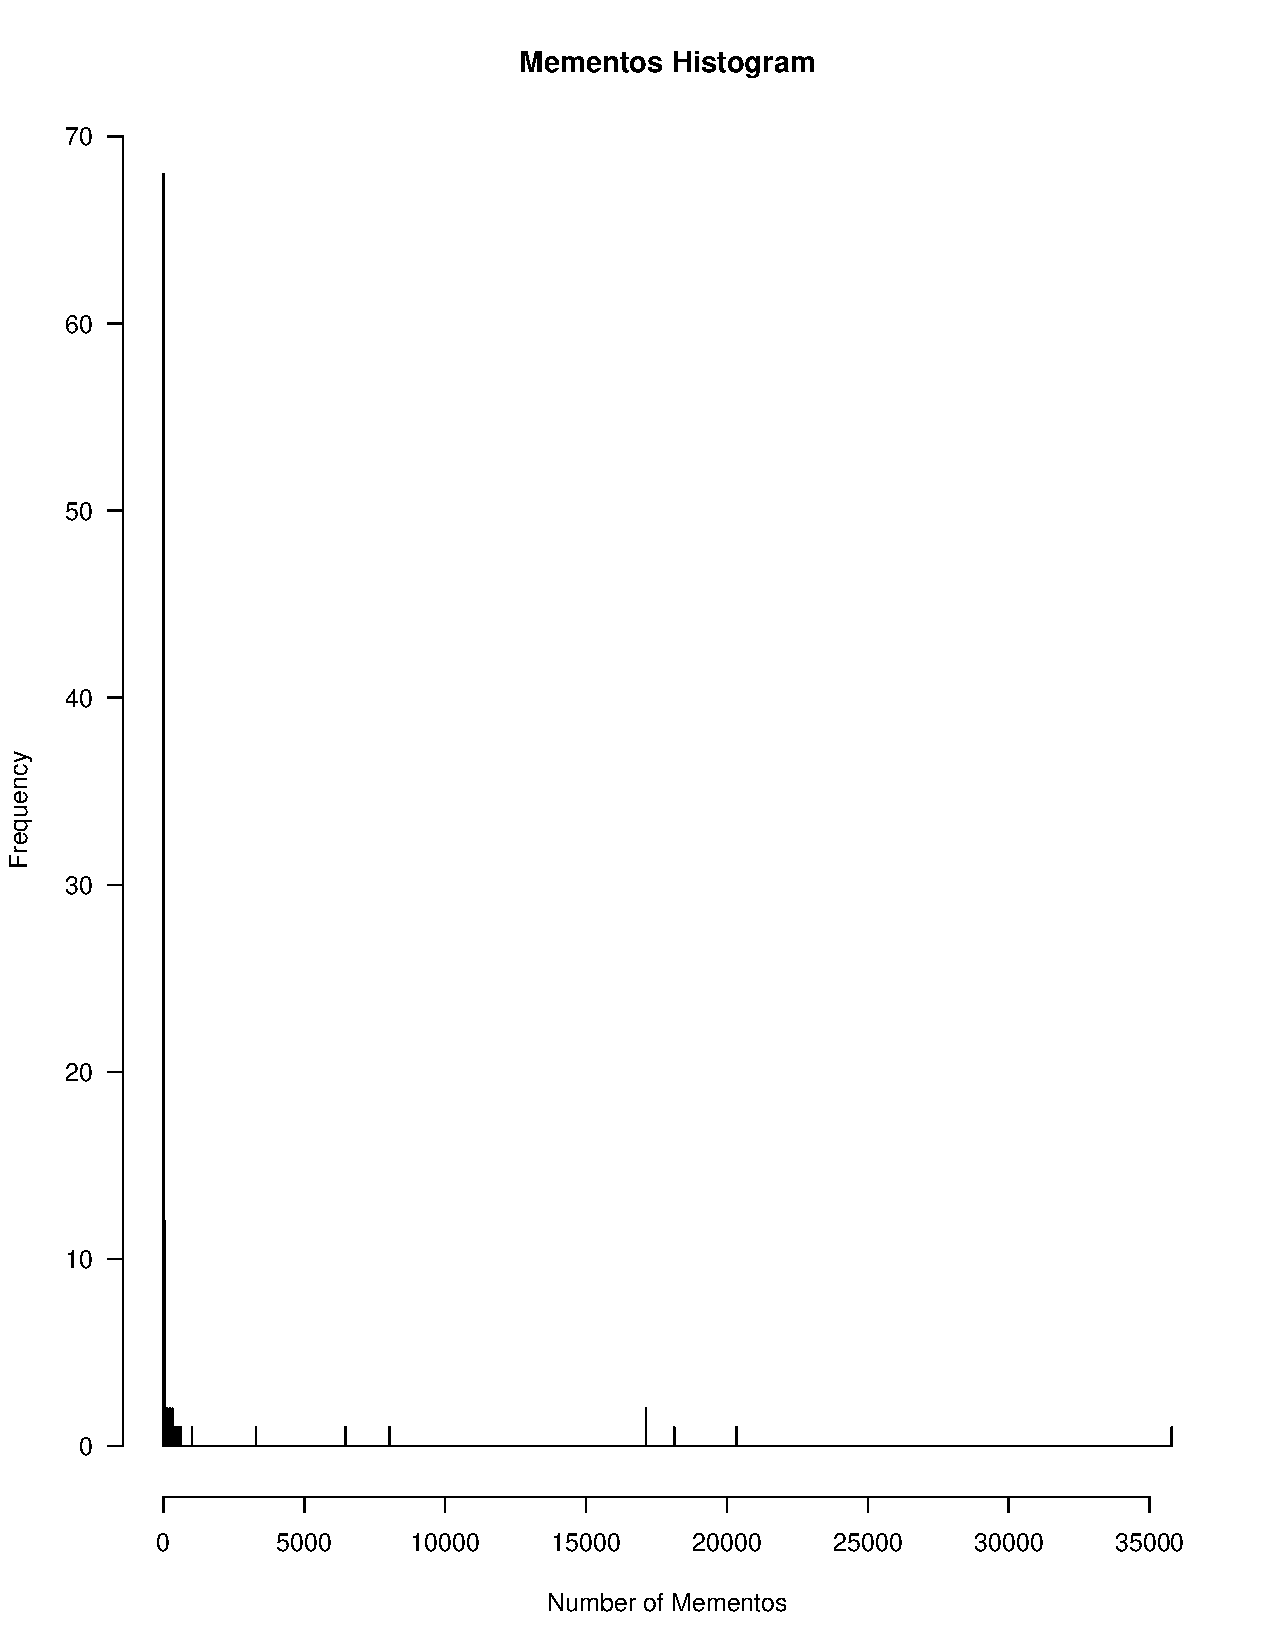
\includegraphics[scale=0.7]{hist1.pdf}
\end{figure}
\pagebreak

We notice that our histogram did not provide a good representation of the results. I am going to zoom into the part where most of the data is and exclude the outliars in the data. Modifying the last line of code to this one will do just that.

\begin{lstlisting}
>  hist(timemaps_data[,1], col=heat.colors(max_num/500), breaks=max_num, xlab="Number of Mementos", xlim=c(0,max_num/500), right=F, main="Mementos Histogram", las=1)
\end{lstlisting}

\begin{figure}[H]
\centering
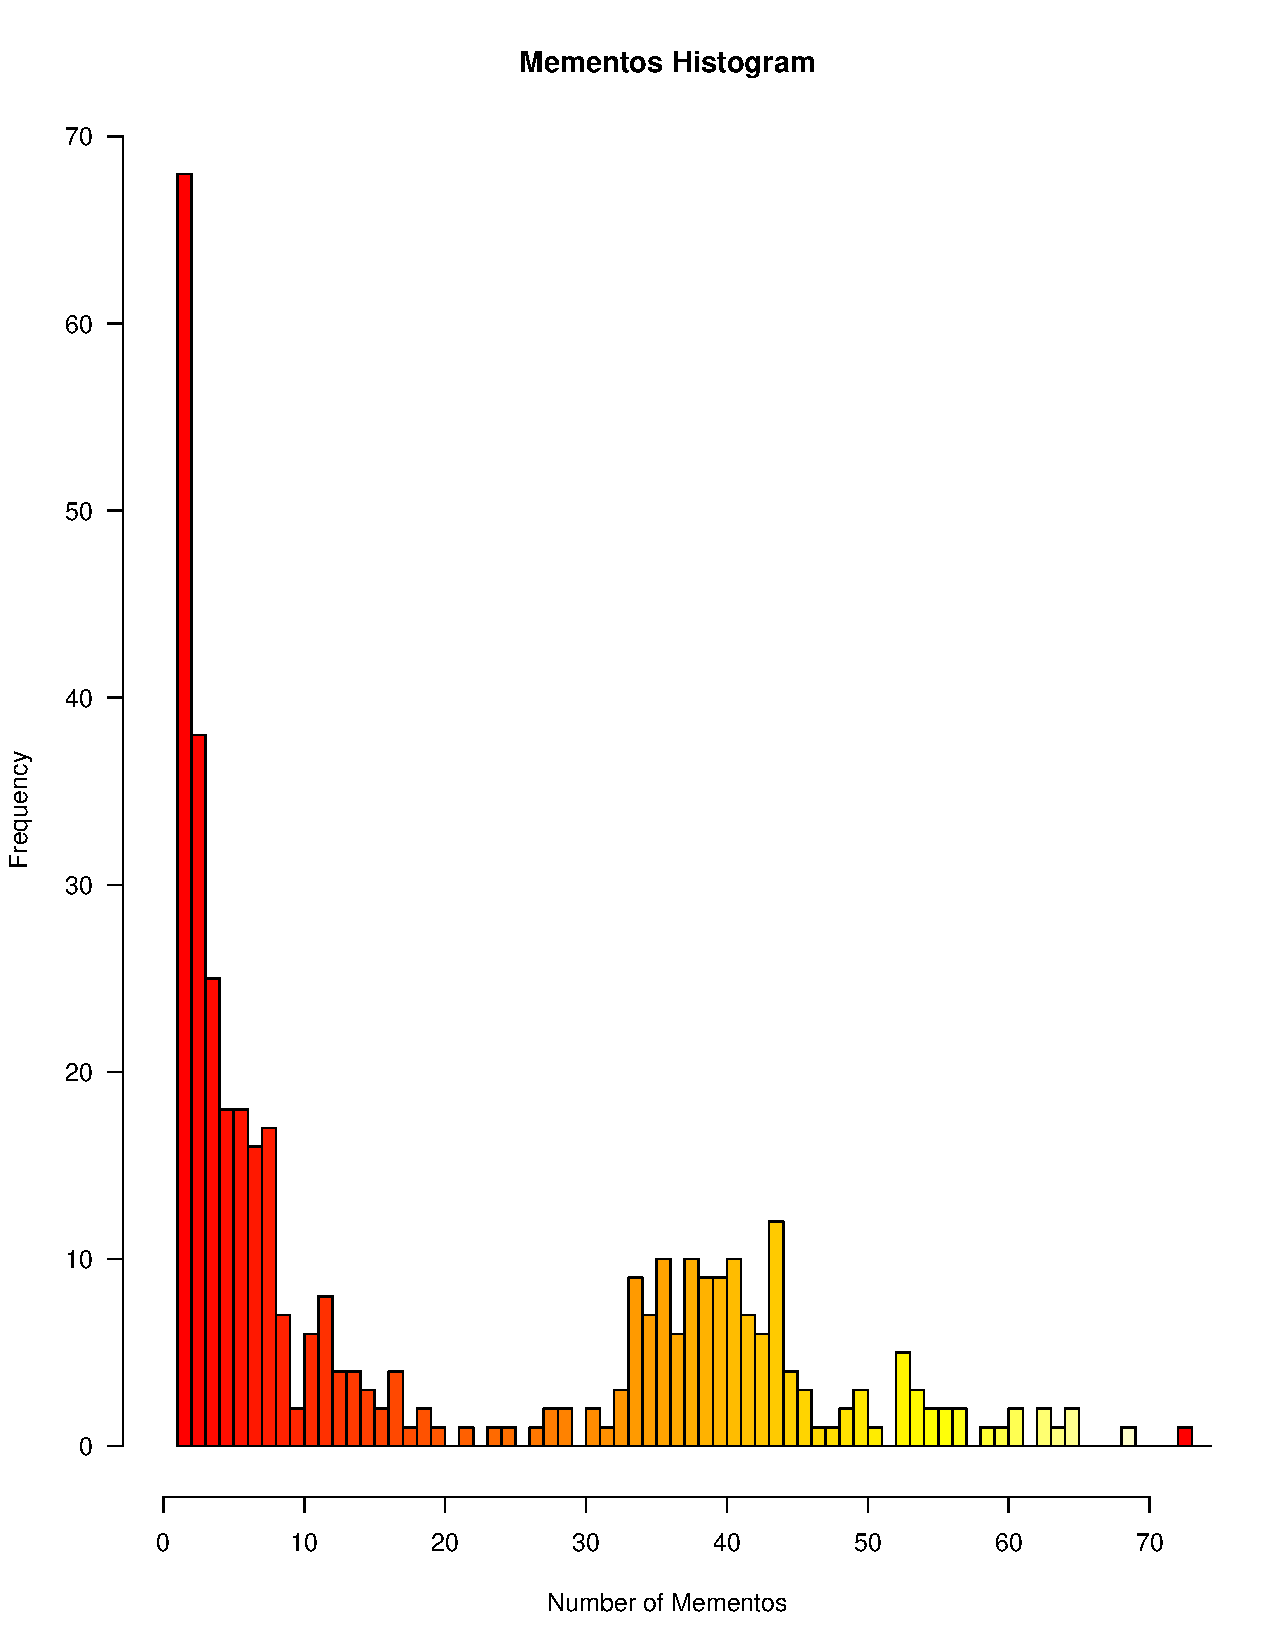
\includegraphics[scale=0.7]{hist2.pdf}
\end{figure}
\pagebreak

The histogram shows that about 68 of the URIs have only one memento and about 38 URIs have two mementos, so on and so forth. It shows that almost half of the URIs, that actually have mementos, have less than 10 mementos.

4. Although this step is not necessary, but I wanted to count the occurrences of each value in ``timemapreport.txt'' and line every unique value with its number of occurrences in a table. From the file ``timemapreport.txt'', generate the data file ``memesvslinks.txt'' that contains our data, number of mementos vs number of links. I wrote a simple script, ``generatelinksvsmemes.py'', that loops over the lines in ``timemapreport.txt'' and generates ``memesvslinks.txt'' by counting the occurrences of each line in ``timemapreport.txt'' and saving the value in the line along with the number of its occurrences.

\lstinputlisting[language=python, label=generatelinksvsmemes.py, caption=The content of generatelinksvsmemes.py, breakatwhitespace=〈false)]{Q2/generatelinksvsmemes.py}

\begin{lstlisting}[language=bash, breakatwhitespace=〈false), label=Command, caption=Running generatelinksvsmemes.py]
root@ima-app:/var/www/Hussam# python generatelinksvsmemes.py timemapreport.txt memesvslinks.txt
root@ima-app:/var/www/Hussam# cat memesvslinks.txt | wc -l
107
root@ima-app:/var/www/Hussam#
\end{lstlisting} 


\subsection*{Included Files:}
downloadtimemapsjson.py, uniquelinks.txt, uniquelinkswithmemes.txt, parsejsontimemap.py, timemapreport.txt, memesvslinks.txt, generatelinksvsmemes.py, bbcmemes.txt, bbcnomemes.txt, hist1.pdf, hist2.pdf 

\noindent 
Folder: timemaps that has all timemap.json* files,  

\section*{Question 3:}
3.  Estimate the age of each of the 1000 URIs using the ``Carbon
Date'' tool:
\burl{http://ws-dl.blogspot.com/2016/09/2016-09-20-carbon-dating-web-version-30.html}

\textbf{Note:} 
you should use ``docker'' and install it locally.  You can do it like this:
\burl{http://cd.cs.odu.edu/cd?url=http://www.cs.odu.edu/}

But it will inevitably crash when everyone tries to use it at the
last minute.

For URIs that have more than 0 Mementos and an estimated creation date,
create a graph with age (in days) on the x-axis and number of
mementos on the y-axis.

Not all URIs will have Mementos, and not all URIs will have an
estimated creation date.  Show how many fall into either categories.
For example:

total URIs:	        1000

no mementos:	 	 137  

no date estimate:	 212
     
\subsection*{Answer:} 

1. To download the estimated creation date for each link in ``uniquelinks.txt'', I wrote a python script, ``downloadcreationdatejson.py'', that does that using the ``Carbon Date'' tool. The script takes two command line arguments, an input file that has the links for which we want to download the estimated creation time ``uniquelinks.txt'', an output file to stores the age of each link (in days) based on the response ``creationreport.txt''.

\lstinputlisting[language=python, label=downloadcreationdatejson, caption=The content of downloadcreationdatejson.py, breakatwhitespace=〈false)]{Q3/downloadcreationdatejson.py}

\begin{lstlisting}[language=bash, breakatwhitespace=〈false), label=Command, caption=Running downloadcreationdatejson.py]
root@ima-app:/var/www/Hussam# Python downloadcreationdatejson.py uniquelinks.txt creationreport.txt
\end{lstlisting}

2. From the first step in the second question, I found out which links has mementos and saved those links in a separate file and named it ``uniquelinkswithmemes.txt''. Now we need to create a program and pass this file as input to see which link has an estimated creation date so we can create a graph with age (in days) on the x-axis and number of mementos on the y-axis. I wrote a python script, ``generatememesvsage.py'' that will take ``uniquelinkswithmemes.txt'' as input and find the number of mementos as well as the age of each link in days and generate the data that necessary to create the graph in R and save it in ``memesvsage.txt'' as output.

\lstinputlisting[language=python, label=generatememesvsage, caption=The content of generatememesvsage.py, breakatwhitespace=〈false)]{Q3/generatememesvsage.py}

\begin{lstlisting}[language=bash, breakatwhitespace=〈false), label=Command, caption=Running generatememesvsage.py]
root@ima-app:/var/www/Hussam# python generatememesvsage.py uniquelinkswithmemes.txt memesvsage.txt
\end{lstlisting} 

The data in ``memesvsage.txt'' is ready to be graphed using R.

3. Now we are ready to generate the scatter plot for the number of mementos vs. the the age in days in R.

This line of code reads the data in the file and stores it in the vector mydf.
\begin{lstlisting}
> mydf <- read.csv2('C:/R/memesvsage.txt', sep = '\t', header = T)
\end{lstlisting}

This line of code generates a basic scatter plot for mementos vs. age.
\begin{lstlisting}
> plot(x = mydf$ageX, y = mydf$memesY, xlab="Age in days",ylab="Number of Mementos",main="Mementos vs Age")
\end{lstlisting}

\begin{figure}[H]
\centering
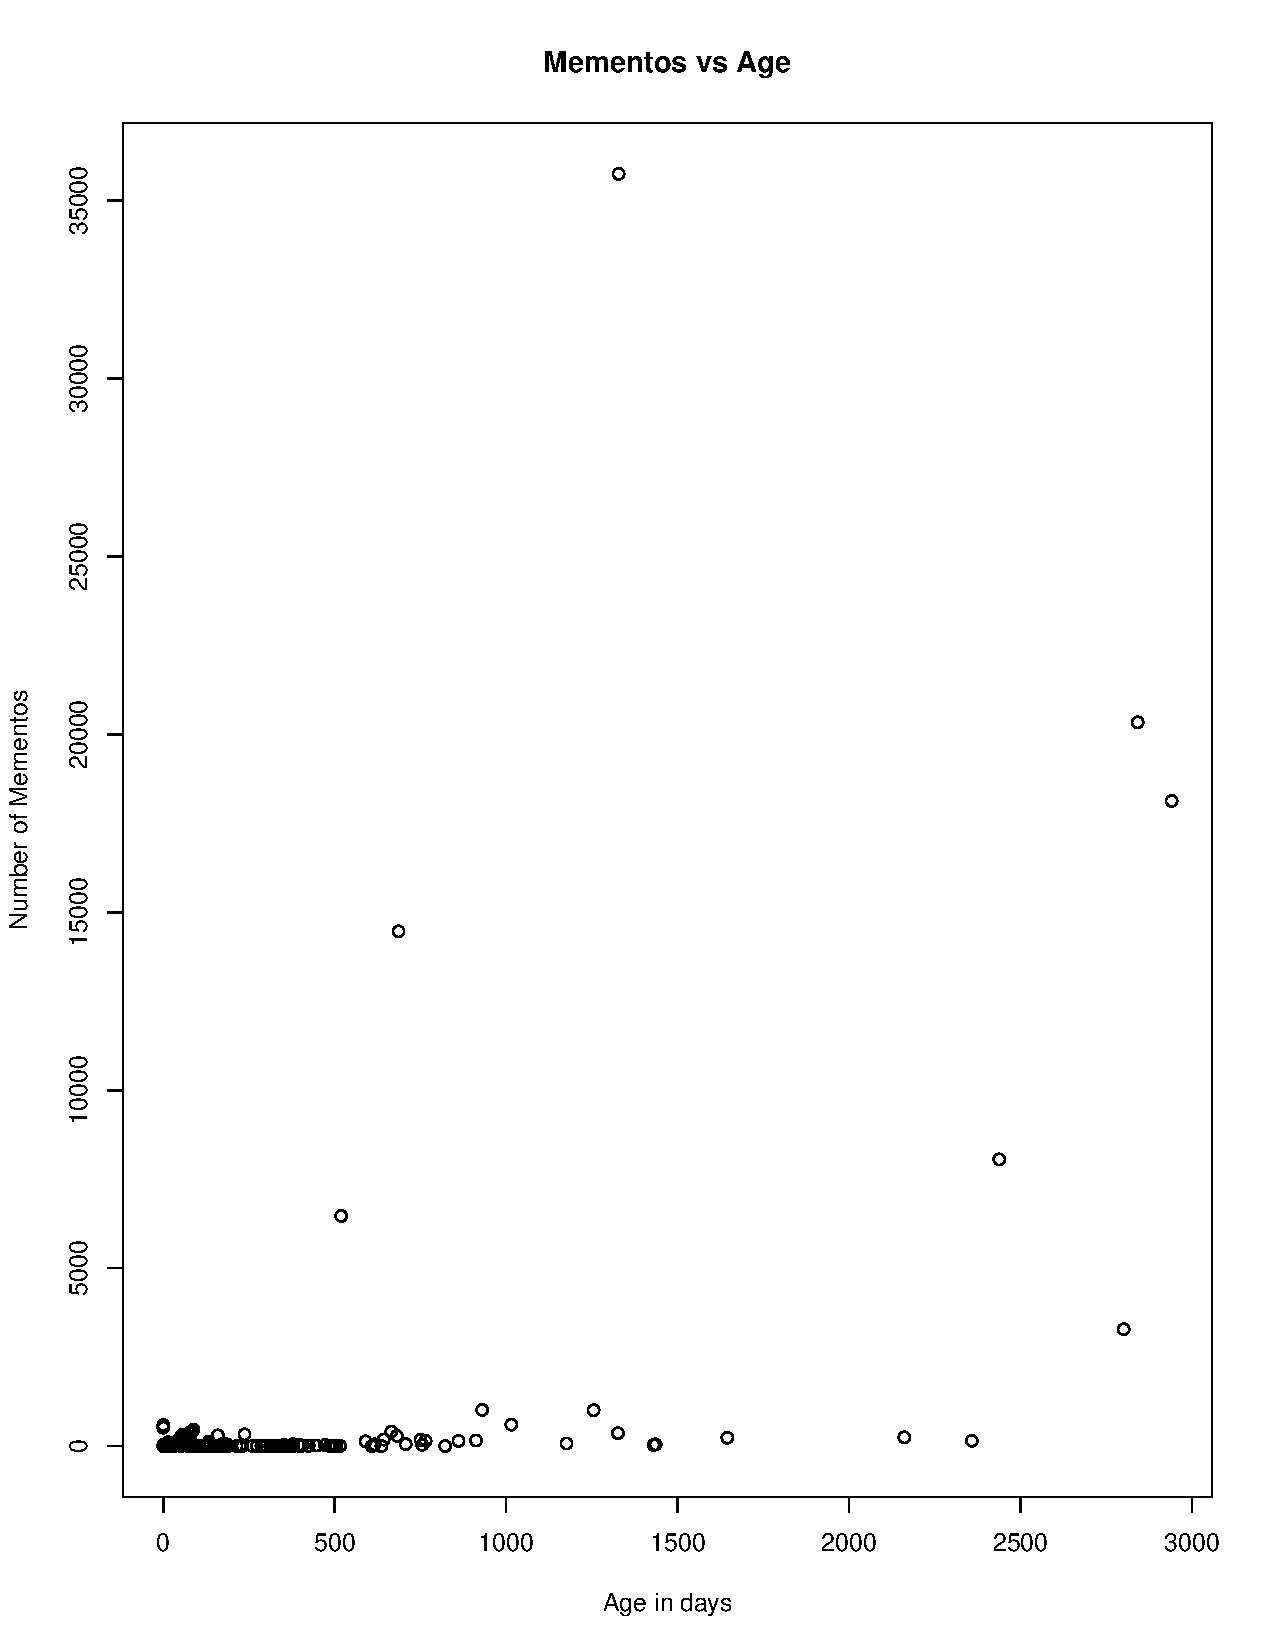
\includegraphics[scale=0.7]{splot1.pdf}
\end{figure}
\pagebreak

Again, I want to zoom in where most of the data is and excluded the outliars, but first let me color code the points based on a simple criteria.

Let's make everything black first:

\begin{lstlisting}
> mydf$Colour="black"
\end{lstlisting}

Points colored in red if the number of mementos is larger than the age in days.

\begin{lstlisting}
> mydf$Colour[mydf$memesY>mydf$ageX]="red"
\end{lstlisting}

Points colored in blue if the number of mementos is smaller than the age in days.

\begin{lstlisting}
> mydf$Colour[mydf$memesY<mydf$ageX]="blue"
\end{lstlisting}

Now this line of code will generate the scatter plot we are looking for:

\begin{lstlisting}
> plot(x = mydf$ageX, y = mydf$memesY,pch=19,xlim=range(1:1000),ylim=range(1:700),xlab="Age in days",ylab="Number of Mementos",main="my title", col=mydf$Colour)
\end{lstlisting}


\begin{figure}[H]
\centering
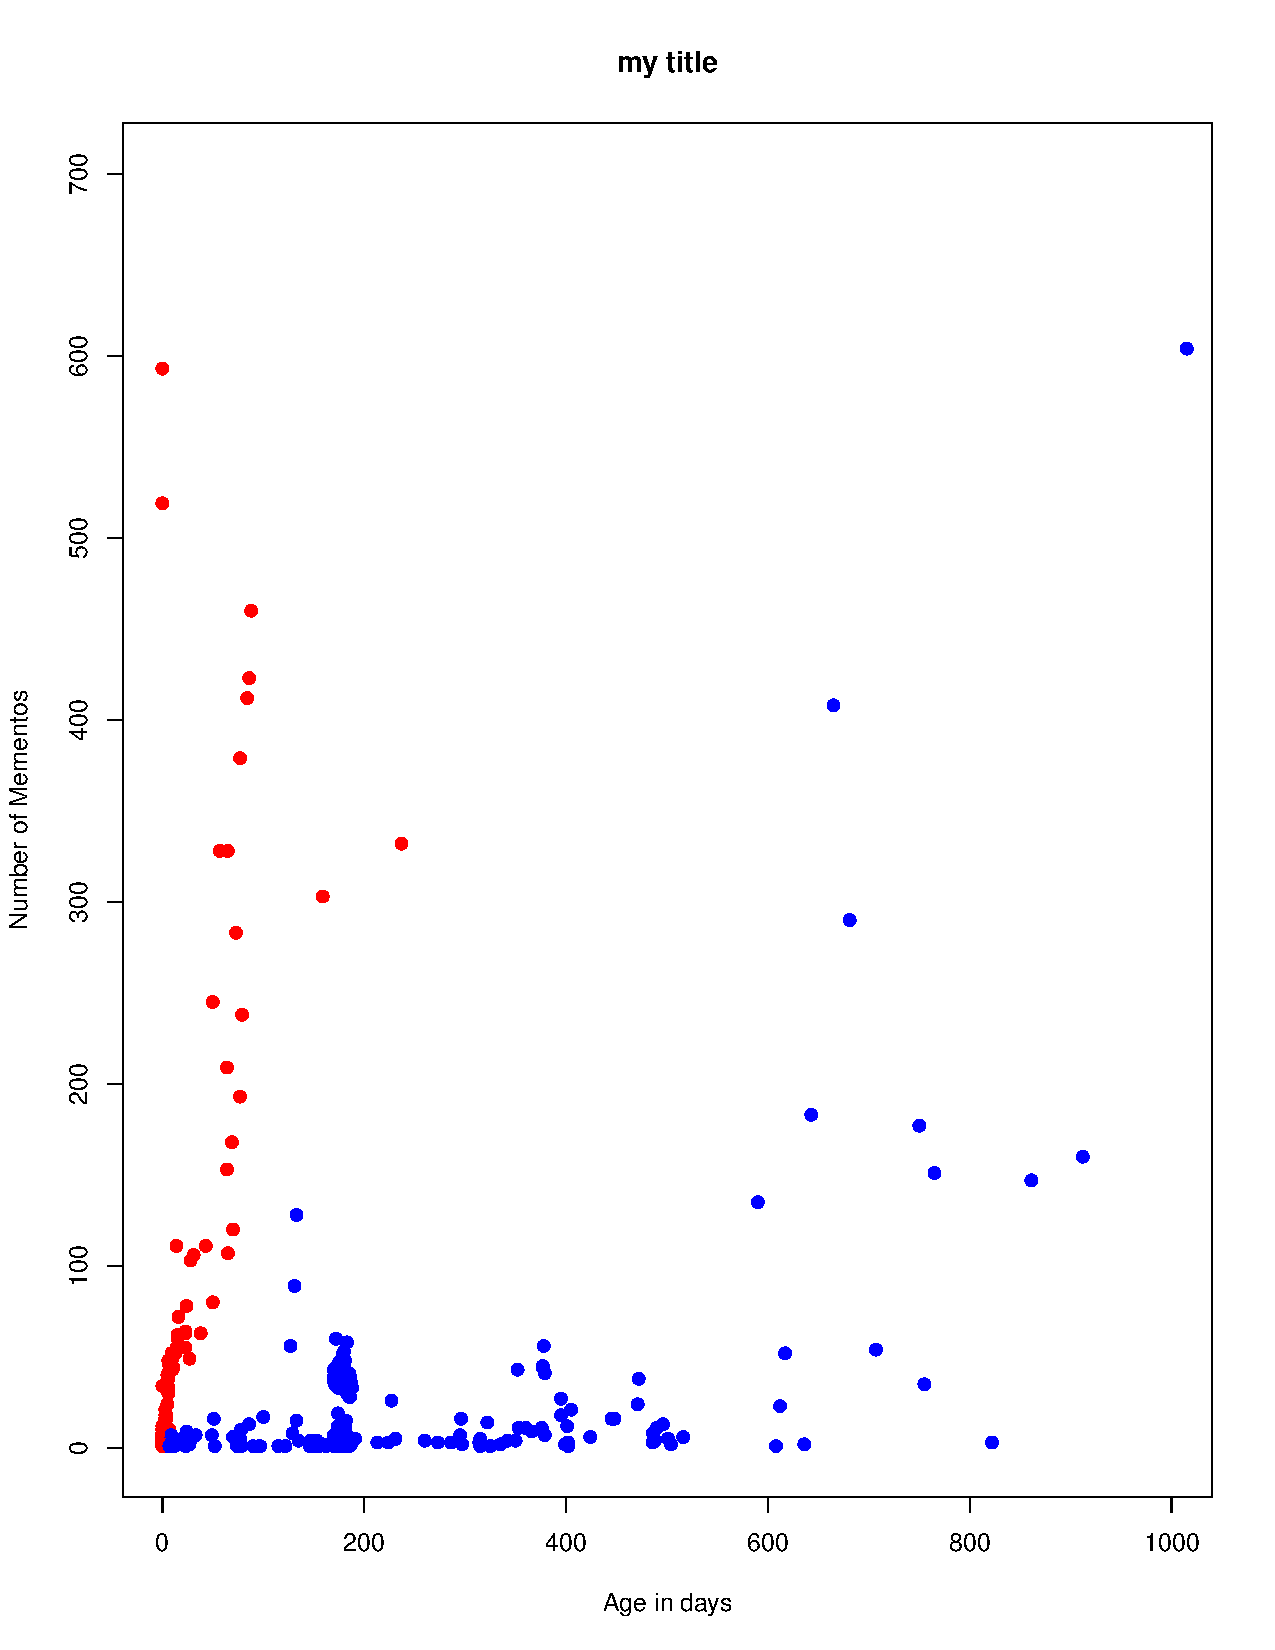
\includegraphics[scale=0.7]{splot2.pdf}
\end{figure}
\pagebreak

\textbf{Conclusion:}
Although the URIs I extracted from Twitter were randomly pulled from different tweets from accounts that belong to news channels, celebrities and so on, it is clear that the data can be represented by a single line using various mathematical algorithms like the least square, and this line is $y = x$. This means that as the age of the URI in days increases, the number of mementos increases, which makes perfect sense.
\linebreak

\textbf{total URIs: 1107}

\textbf{no mementos: 662}  

\textbf{no date estimate: 6}

\subsection*{Included Files:}
downloadcreationdatejson.py, generatememesvsage.py, memesvsage.txt, uniquelinks.txt, uniquelinksage.txt, uniquelinkswithmemes.txt, splot1.pdf, splot2.pdf

\pagebreak


\begin{thebibliography}{9}
\bibitem{knuthwebsite} 
Harding University: Producing Simple Graphs with R by Frank McCown
\\\texttt{http://stackoverflow.com/questions/tagged/python}

\bibitem{knuthwebsite} 
Old Dominion University: Plotting in R by Martin Klein
\\\texttt{http://www.cs.odu.edu/~mklein/cs796/lecture/plotting.html}
 
\bibitem{knuthwebsite} 
Stack Overflow: Python
\\\texttt{http://stackoverflow.com/questions/tagged/python}

\bibitem{knuthwebsite} 
Stack Overflow: R
\\\texttt{http://stackoverflow.com/questions/tagged/r}

\end{thebibliography}



\end{document}
